\documentclass[12pt,prb,aps,epsf]{article}
\usepackage[utf8]{inputenc}
\usepackage{amsmath}
\usepackage{amsfonts}
\usepackage{amssymb}
\usepackage{graphicx} 
\usepackage{latexsym} 
\usepackage[toc,page]{appendix}
\usepackage{listings}
\usepackage{xcolor}
\usepackage{soul}
\usepackage[T1]{fontenc}
\usepackage{amsthm}
\usepackage{mathtools}
\usepackage{setspace}
\usepackage{array,multirow,makecell}
\usepackage{geometry}
\usepackage{textcomp}
\usepackage{float}
%\usepackage{siunitx}
\usepackage{cancel}
%\usepackage{tikz}
%\usetikzlibrary{calc, shapes, backgrounds, arrows, decorations.pathmorphing, positioning, fit, petri, tikzmark}
\usepackage{here}
\usepackage{titlesec}
%\usepackage{bm}
\usepackage{bbold}

\geometry{hmargin=2cm,vmargin=2cm}

\begin{document}
	
	\title{MP 29 Ondes, propagation et conditions aux limites}
	\author{Maria}
	
	\maketitle
	
	\tableofcontents
	
	\pagebreak
	
\section{Propagation d'une onde dans l'air}
On a un émetteur relié à un GBF délivrant un signal de fréquence 40kHz, qui transmet l'ultrason vers un récepteur. On va alors regarder le déphasage entre signal reçut à l'oscillo en fonction de la distance entre émetteur et récepteur, cela permettant de déterminer la longueur d'onde de l'onde transmise. Dans la pratique on trace L(nombre de noeuds $n$) et on modélise par une droite pour obtenir $\lambda$ car on aura $L=\lambda n$. On en déduit ainsi la vitesse du son dans l'air puisqu'on connaît la fréquence du signal, selon
\begin{eqnarray}
c=\lambda f
\end{eqnarray}
\paragraph{Remarque :} Pour pointer les nœuds il est judicieux de se placer en mode XY avec l'oscillo, car beaucoup plus précis.
\paragraph{Point physique} ici on impose une période temporelle et on oserve que cela induit une périodicité spatiale, qui traduit la relation de dispersion $\lambda =cT$. On a ce que l'on appelle la double périodicité, qui est très générale.

\paragraph{Remarque :} on a toujours, pour les ondes matérielles 
\begin{eqnarray}
c^2 = \frac{raideur}{masse} \left(\stackrel{son\;dans\;l'air}{=} \;\;\frac{\gamma R T}{\mu}\;\; \stackrel{deformation\;corde}{=} \frac{T}{\mu} \right)
\end{eqnarray}
plus le milieu est rigide plus l'onde va vite, plus les particules à mettre en mouvement sont lourdes plus elle va lentement.

\section{Corde de Melde : mauvais titre $\rightarrow$ C.L : spectre des modes propres}
On a une corde fixée à l'une extrémité à l'aide d'une masse et d'une poulie, cela permettant de connaître la tension appliquée, et de l'autre à un électro-aimant dont on fixe la fréquence de vibration avec un GBF amplifié en courant (GBF basse impédance 0.5$\Omega$). On connait la longueur L de la corde, et on connait donc, en fonction de sa masse linéique calculée auparavant, les fréquences propres d'oscillation de la corde.\\
On va ici se placer en régime forcée puisqu'on impose la fréquence de vibration avec l'électro-aimant, et constater un phénomène de résonance en amplitude lorsque la fréquence du forçage sera égale à une des fréquences propres du système. Pour cette fréquence la puissance transmise au signal sera alors optimale : définition de la résonance.\\

Dans la pratique on va tracer la fréquence de résonance en fonction de n, un entier repérant chacun des modes. On obtient une droite 
\begin{eqnarray}
f_n = \frac{c}{2L}n
\end{eqnarray} 
permettant de remonter à la vitesse de propagation de l'onde de déformation de la corde par exemple, ou à la densité linéique selon
\begin{eqnarray}
\mu_{exp} = \frac{T}{c^2}
\end{eqnarray}

\begin{figure}
	\centerline{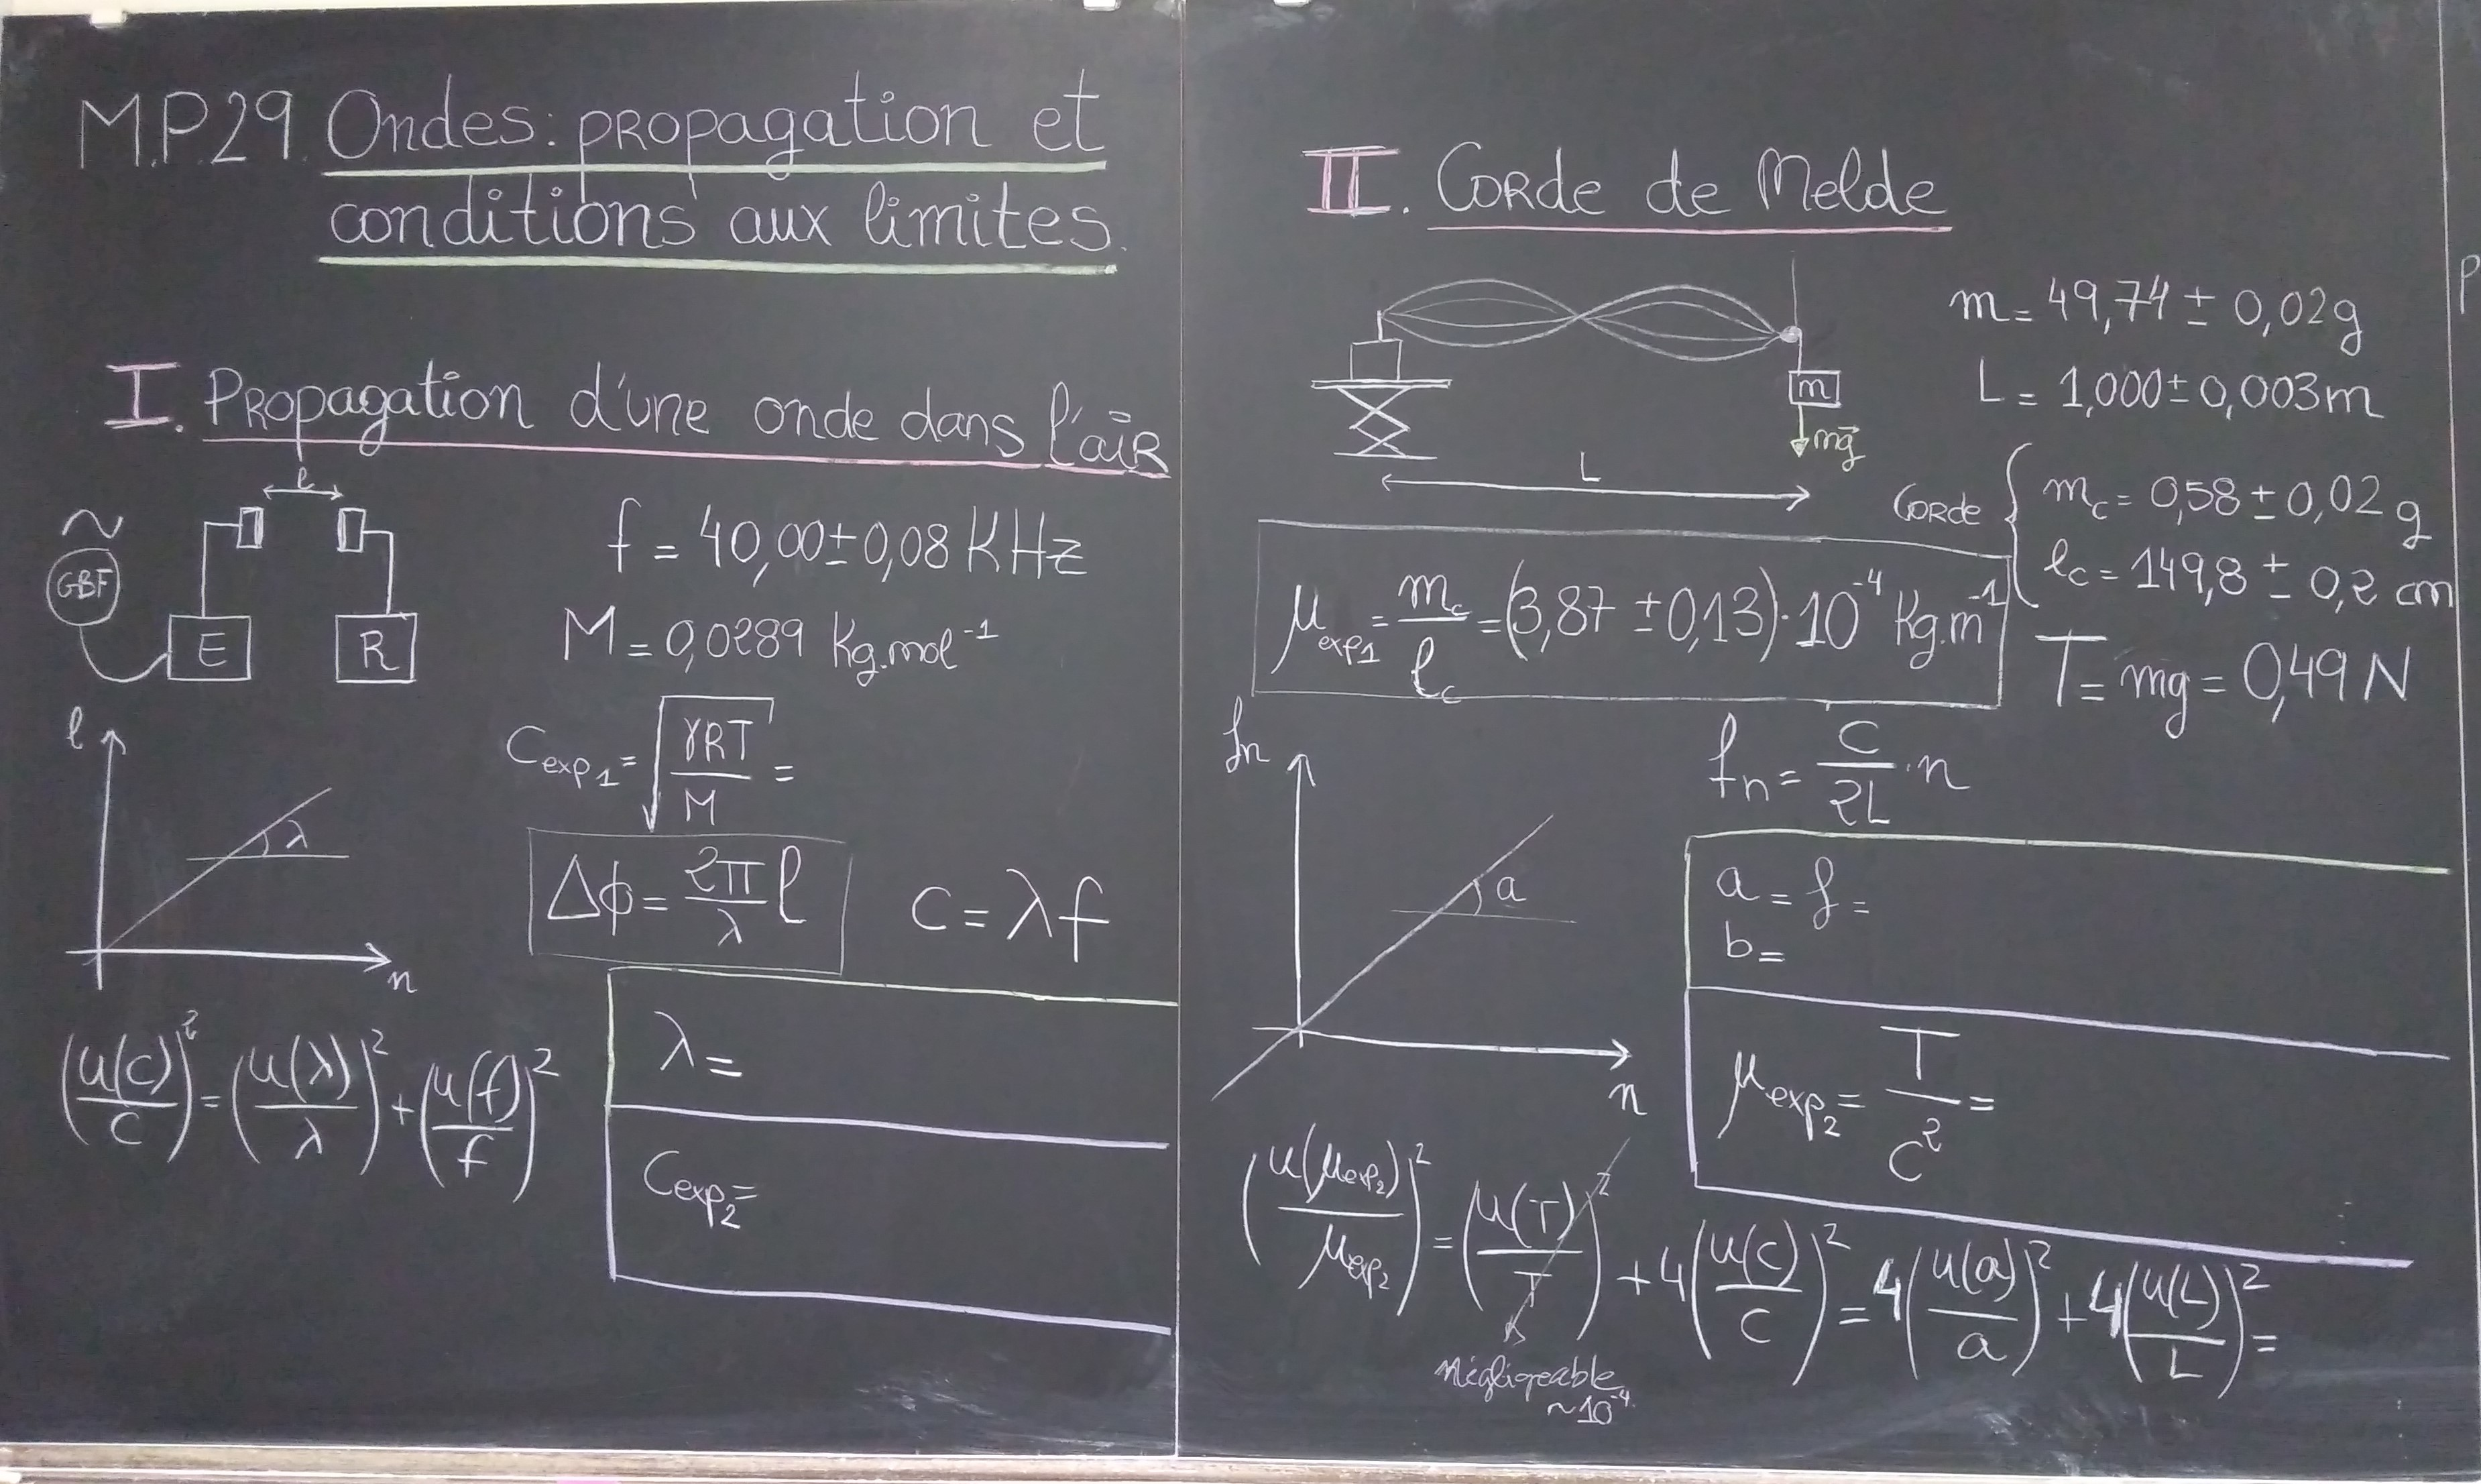
\includegraphics[width=17cm]{T1}}
\end{figure}

\paragraph{Point physique} ici on a en réalité résonance = interférences constructives entre onde incidente et onde réfléchie : on a alors une onde stationnaire d'amplitude maximale. Cette notion est universelle : elle décrit toute les cavités et les puits de potentiels. On peut par exemple la lier au cas de l'atome d'hydrogène qui correspond au cas d'un électron dans un potentiel harmonique.

\section{Câble coaxial}
On peut modéliser le câble coaxial à l'aide de composants linéaires formant un motif se répétant le long du câble. On en déduit une équation de propagation pour la tension et le courant, avec ainsi l'apparition d'une vitesse de propagation. On peut mesurer celle ci en regardant le déphasage entre un signal incident et un signal réfléchi au bout d'un câble coax de longueur  $L=50$ m : $v = \frac{2L}{\Delta t}$.\\

On a plusieurs cas de C.L : 

$z=\infty$ : circuit ouvert (pas de bouchon), onde réfléchie.\\

$z=0$ court circuit, onde réfléchie en sens inverse $\rho = \frac{z-z_c}{z+z_c}$\\

$z=z_c$ adaptation d'impédance (bouchon de même impédance que le câble).\\
On peut ainsi remonter à la capacité linéique du câble
\begin{eqnarray}
\Gamma_{th} = \frac{2\pi\varepsilon\varepsilon_r}{2u\frac{b}{a}}\\
\Gamma _{exp} = \frac{1}{v\,z_c}
\end{eqnarray}

\paragraph{Point physique} Là encore on a un milieu décrit par l'équation de d'Alembert, qui est ainsi non dispersif, ce qui se vérifie pour la réflexion : le pic réfléchi fait la même taille que le pic envoyé.

\section{Diffraction}	
On éclaire une fente à l'aide d'un laser et on mesure la position l de chaque frange sombre n (à partir d'une origine arbitraire) et on trace ensuite $l(n)$. La modélisation affine permet alors de remonter à l'épaisseur des franges, cette dernière étant directement liée (lorsqu'on est dans les conditions de Fraunhofer $D\gg\frac{a^2}{\lambda}$) à la largeur de la fente a selon
\begin{eqnarray}
a = \frac{\lambda D}{l}
\end{eqnarray}
où D est la distance entre la fente et l'écran, et où la longueur d'onde $\lambda$ du laser peut être mesurée à l'aide d'un spectromètre.\\
On peut comparer la largeur de fente obtenue à la valeur mesurée à l'aide d'un microscope.

\paragraph{Point physique} On montre en fait ici que l'impulsion est la variable conjuguée de la variable position, on met en évidence le principe d'incertitude de Heisenberg : on contraint la position et alors on génère une indétermination sur l'impulsion.

\begin{figure}
	\centerline{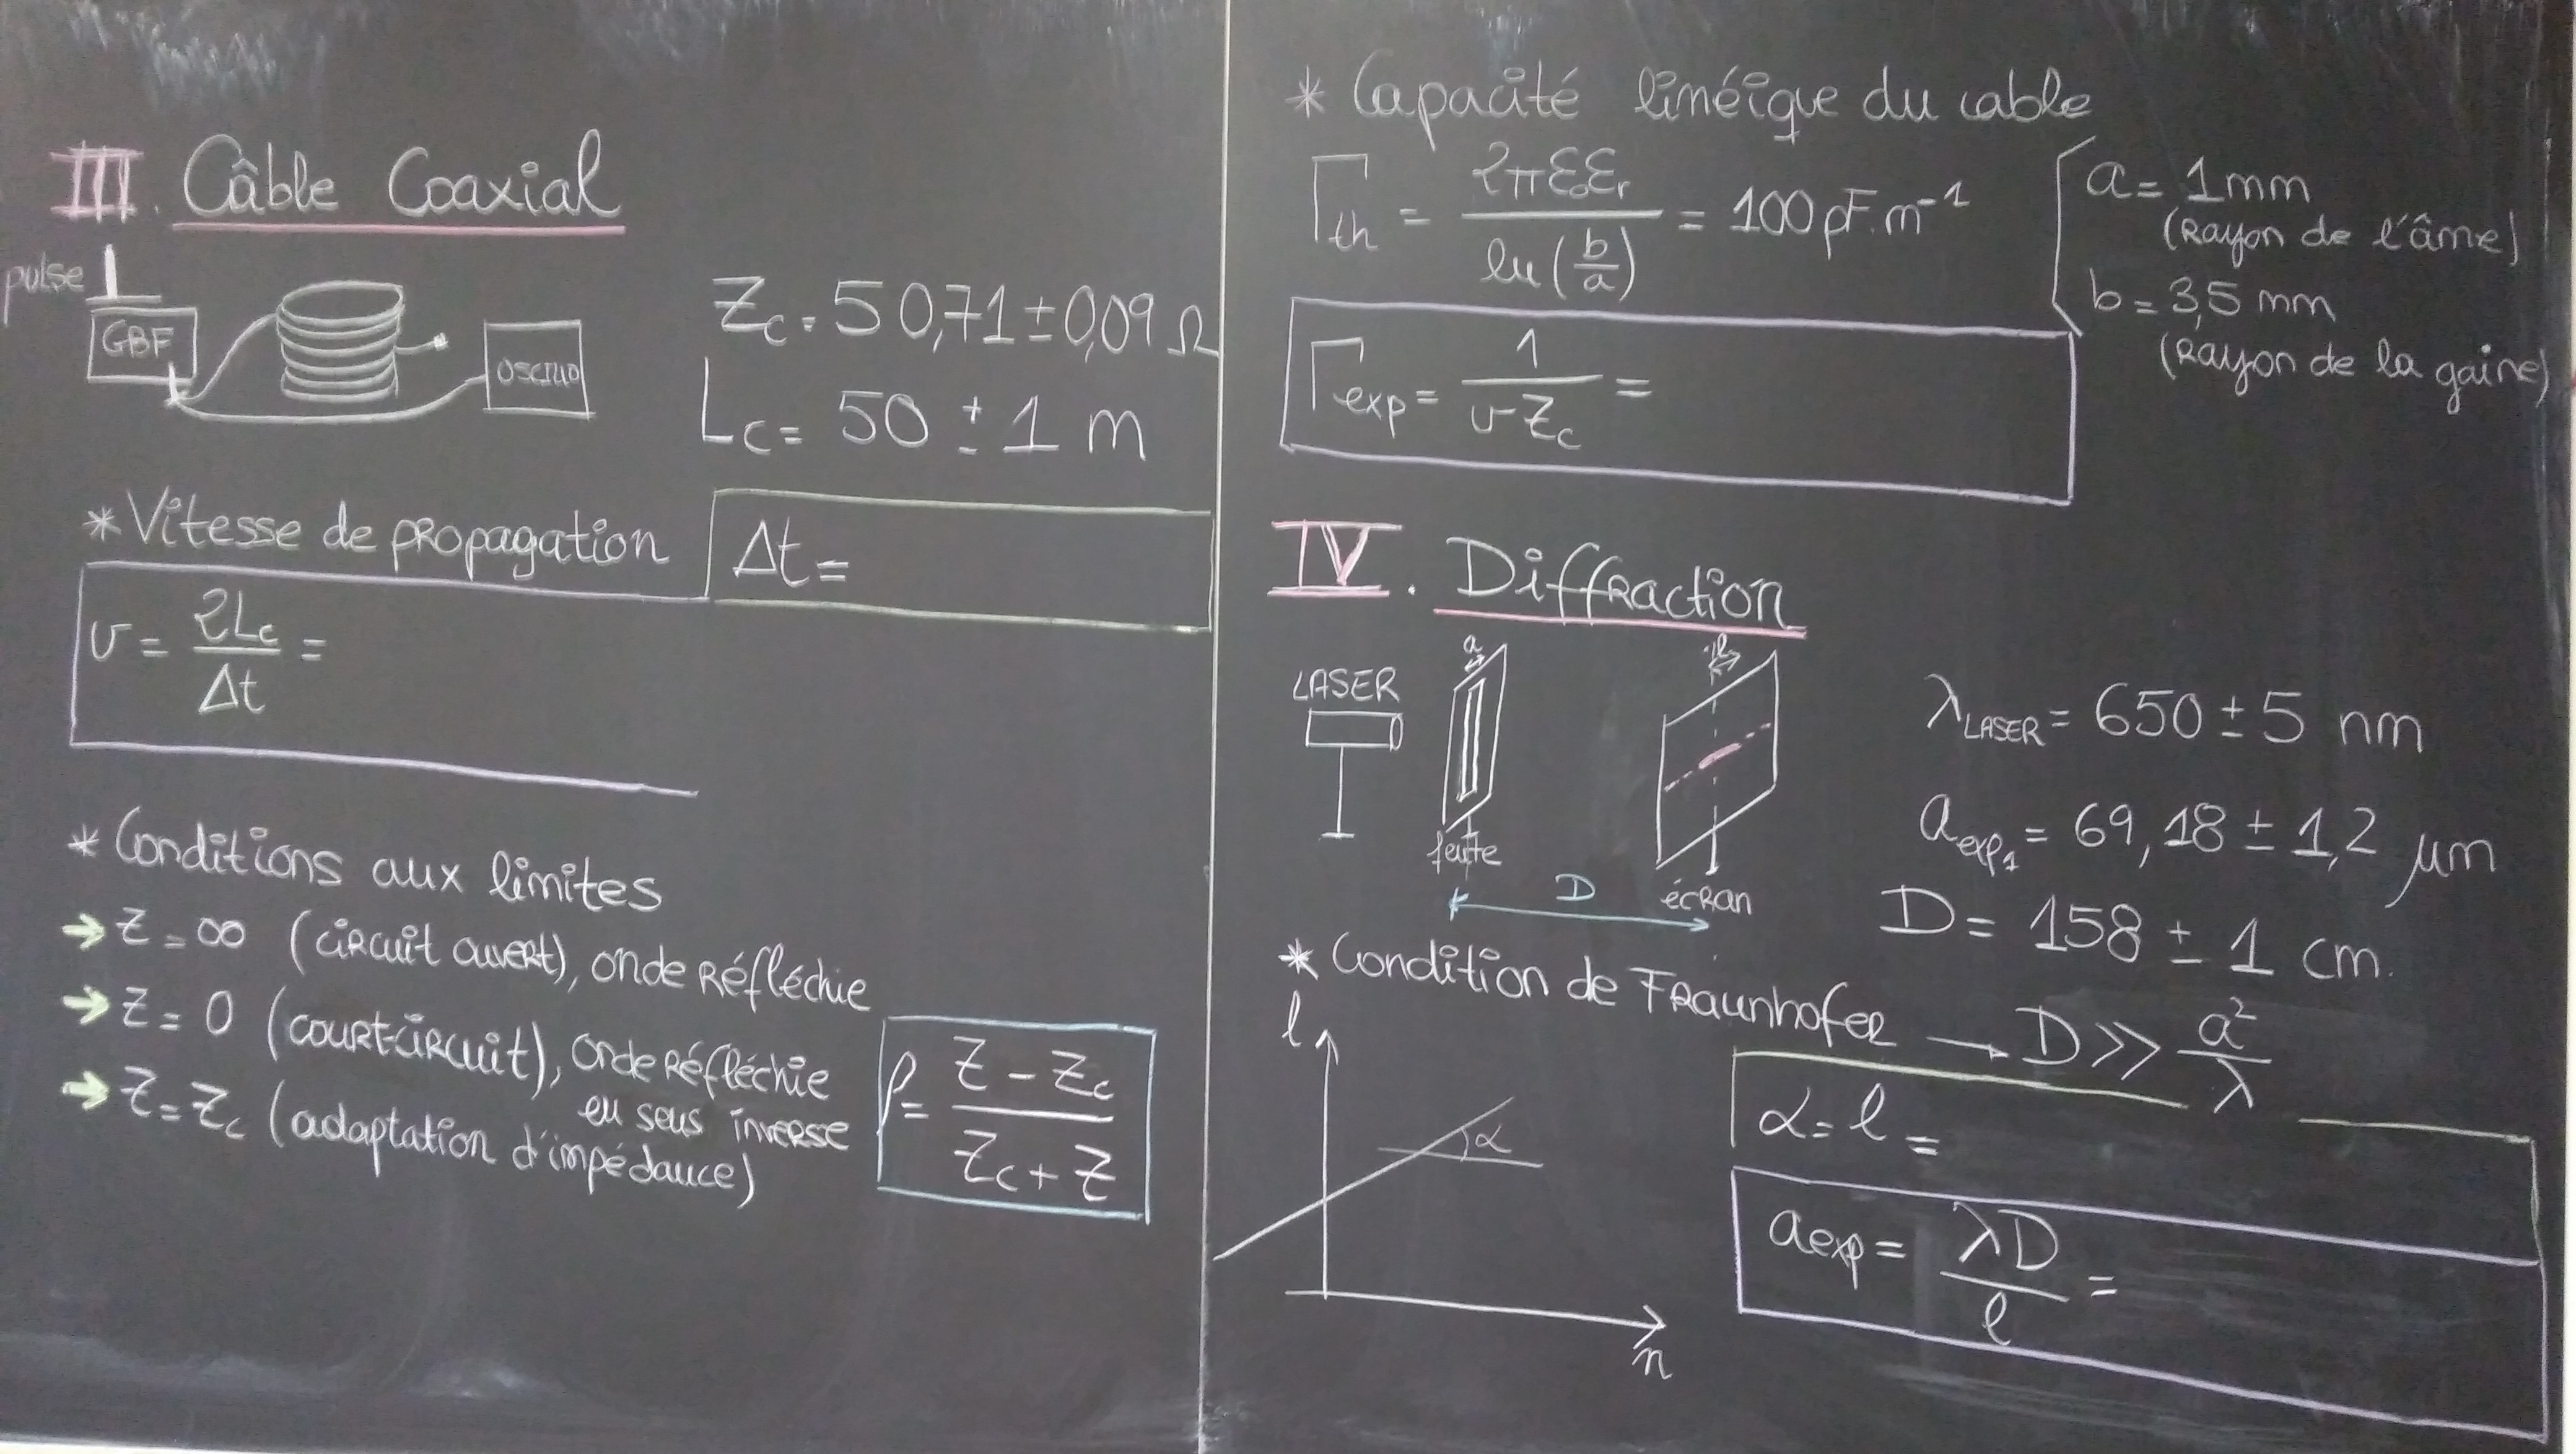
\includegraphics[width=17cm]{T2}}
\end{figure}

\section*{Questions}
Concernant le laser, l'incertitude donnée par le constructeur est de quelle nature ?\\

Pouvez vous commenter la validité de l'approximation de Fraunhofer ici ?\\
On voit qu'on aura ici une erreur théorique de un pour cent.\\

Comment se placer dans un cadre permettant de ne pas avoir cette erreur ?\\
On prend une fente plus petite ou on regarde à l'infini à l'aide d'une lentille bien placée.\\

Qu'observe t-on si on place, à la place du bouchon, une boite à décade réglée de telle sorte à avoir une résistance $R=z_c$ ? Explication ? Pourquoi cela diffère du bouchon ?\\
On a un truc du type dérivateur, il y a donc une capactité. En fait à haute fréquence (au dela de 10kHz) la résistance se comporte comme une capacité, ce qui est le cas ici puisqu'on envoie un pulse : constitué d'harmoniques hautes fréquence. Le bouchon est quand à lui fait pour demeurer une résistance de 50$\Omega$ même ç haute fréquence.\\

Pour la mesure de la résistance du bouchon à l'Ohmètre, à quelle fréquence est elle effectuée ?\\
à fréquence nulle : continu.\\

Cela a t'il du sens de comparer une impédance mesurée à fréquence nulle et une impédance mesurée à haute fréquence ?\\

Concernant la corde de Melde, vous mesurée une masse linéique ... est ce comme ça qu'on calcule une masse linéique ?\\

Vu le titre du montage, cette mesure est elle pertinente ? Qu'apprend on sur les ondes ?\\

Ce phénomène est il spécifique à la corde ?\\


	
	
	
\end{document}